\section{Proposition}
Pour créer la sortie de corps dans le but d'aider les patients atteints d'anorexie mentale, nous devons respecter deux critères. Tout d'abord la synchronisation entre ce qui est vu dans le virtuel et perçu dans la réalité est essentiel pour créer le phénomène de sortie de corps en réalité virtuelle. Ensuite, le contexte applicatif du sujet, nous contraint d'utiliser du matériels à bas prix.\\

Pour mettre au point une application permettant d'induire la sensation de sortie de corps, nous allons nous inspirer du principe notamment utilisé par Lopez et al. \cite{bl10} en utilisant un stimuli tactile qui affecte à la fois le vrai corps et le corps virtuel telle que le bâton qui touche le sujet pendant que celui-ci vois une vidéo en direct de lui touché par ce même bâton. Pour avoir un impact sur la perception de l'apparence de son corps, nous allons reprendre l'idée décrite par Preston et al. \cite{pr14}. Dans leur article, ils décrivent la manière dont ils ont pu modifier la satisfaction que les personnes ont de leurs corps grâce à une sortie de corps partielle au niveau du ventre et avec des mannequins de différentes corpulences. Dans notre cas nous souhaitons réaliser cela avec une sortie de corps complète permettant ainsi d'avoir un impact sur la perception qu'ils ont de leurs bras et jambes. Pour obtenir plus de liberté dans l'apparence du corps virtuel et aussi dans sa modification, nous allons réalisé cette sortie de corps dans un environnement virtuel 3D qui sera vu via un casque de réalité virtuelle et des modèles 3D de corps humain.\\

Pour créer la sensation de sortie de corps, nous avons décidés de nous baser sur deux principes, la corrélation visuotactile et la corrélation visuomotrice entre le monde réel et le monde virtuel dans le but de perturber le processus d'intégration multisensorielle.\\

\begin{figure}[!h]
   	\centerline{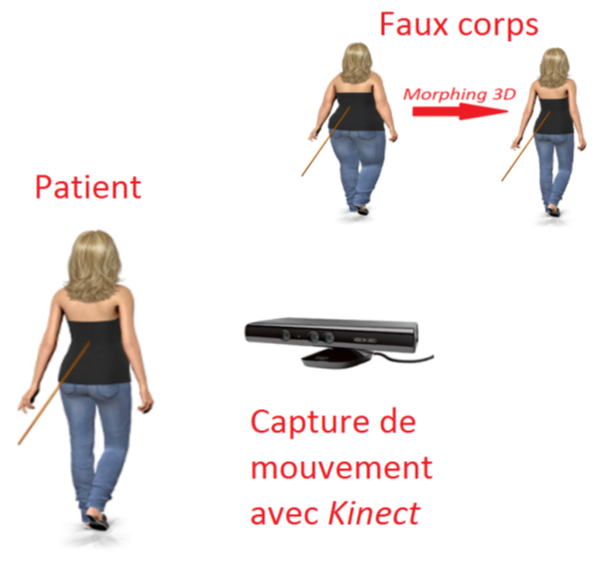
\includegraphics[scale=0.8]{images/schemaProposition}}
   	\caption{\label{fig10} Schéma de l'application proposée}
\end{figure}

La corrélation visuomotrice, c'est à dire le lien entre ce qui est vu et les mouvements que l'on fait, est réalisée grâce à la capture de mouvement en temps réel qui permet à l'avatar de reproduire les mouvements réalisés par l'utilisateur. la corrélation visuotactile, lien entre ce qui est vu et ce qui est ressenti par l'utilisateur, est fait en se servant d'un bâton qui viendra touché le sujet et dans le monde virtuel, un bâton viendra également toucher l'avatar en reproduisant les mouvements du bâton réel. Comme dans certains des travaux vu précédemment, nous avons décidé de choisir le dos pour être la zone sur laquelle seront réalisée les stimulations tactiles. Il faut donc que dans le monde virtuel, l'utilisateur voit son avatar de dos (Voir Figure \ref{fig10}). Ces deux points sont donc réalisés grâce à la capture de mouvement, ceux du sujet et ceux du bâton. La capture de mouvement de l'utilisateur sera réalisée via la \emph{Microsoft Kinect} car elle propose une capture de mouvement de bonne qualité par rapport à son coût. Pour capturer les mouvements du  bâton, nous utiliserons la \emph{Razer Hydra} car elle offre une bonne précision tout en restant abordable et comme l'expérimentateur sera celui qui utilisera cet appareil, le fait qu'il s'agit d'un système intrusif n'est pas un problème.\\

\begin{figure}[!h]
   	\centerline{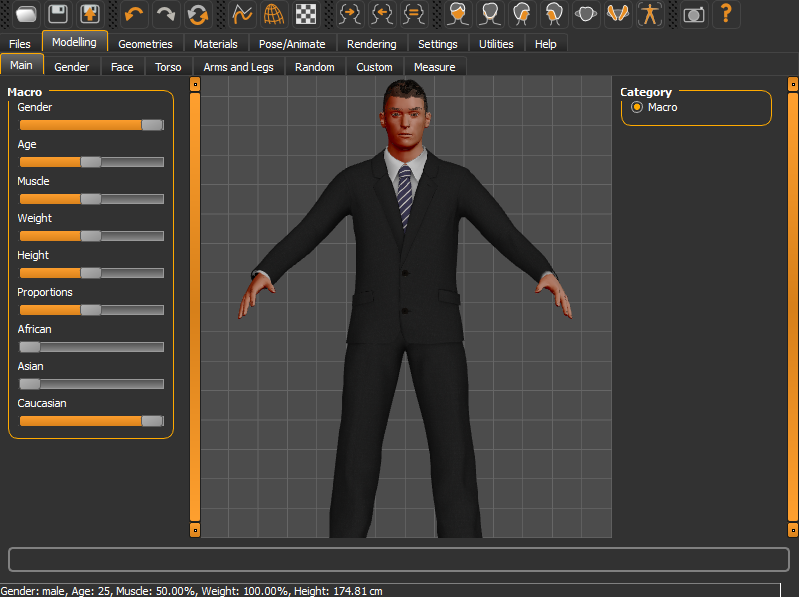
\includegraphics[scale=0.4]{images/makeHuman}}
   	\caption{\label{fig11} Interface de \emph{MakeHuman}}
\end{figure}

Pour l'avatar contrôlé par l'utilisateur, nous avons décidé de proposer aux patients une large gamme de modèles avec les mêmes caractéristiques (cheveux, vêtements, visage ...) mais avec des corpulences différentes. Les différents modèles seront créés avec \emph{MakeHuman}\footnote{www.makehuman.org}. Nous avons choisi ce programme car, en plus d'être open-source et sous licence CC0, il offre un large ensemble d'options pour modifier l'apparence d'un modèle en ce qui concerne la corpulence de son corps (Voir Figure \ref{fig11}). Ainsi il est possible de modifié la masse corporelle et la masse musculaire, ou de modifier chaque membre un par un. Comme tout nos modèles seront proches et fait à partir du même logiciel, il est facile de s'assurer que tout nos avatar aient les mêmes caractéristiques technique tel que le même nombre de points pour définir la forme des modèles et les mêmes textures. On peut aisément utiliser le \emph{Morphing 3D} pour créer la déformation d'un avatar vers un autre.\\

Ainsi la première étape sera que le sujet choisisse l'avatar qui lui ressemble le plus en terme de corpulence puis l'expérimentateur pourra choisir un autre avatar. Ensuite l'utilisateur verra l'avatar choisit de dos dans une simple scène 3D représentant une pièce classique. L'expérimentateur commencera alors à toucher le sujet dans le dos pendant que le bâton virtuel fera la même chose sur l'avatar. En même temps, le corps virtuel se transformera progressivement jusqu'à avoir l'apparence du modèle choisi par l'expérimentateur. 
